\documentclass[12pt, fleqn]{article}
\usepackage{./course_style}

\begin{document}

\begin{titlepage}
    \begin{center}
        Московский государственный университет имени М. В. Ломоносова
        
        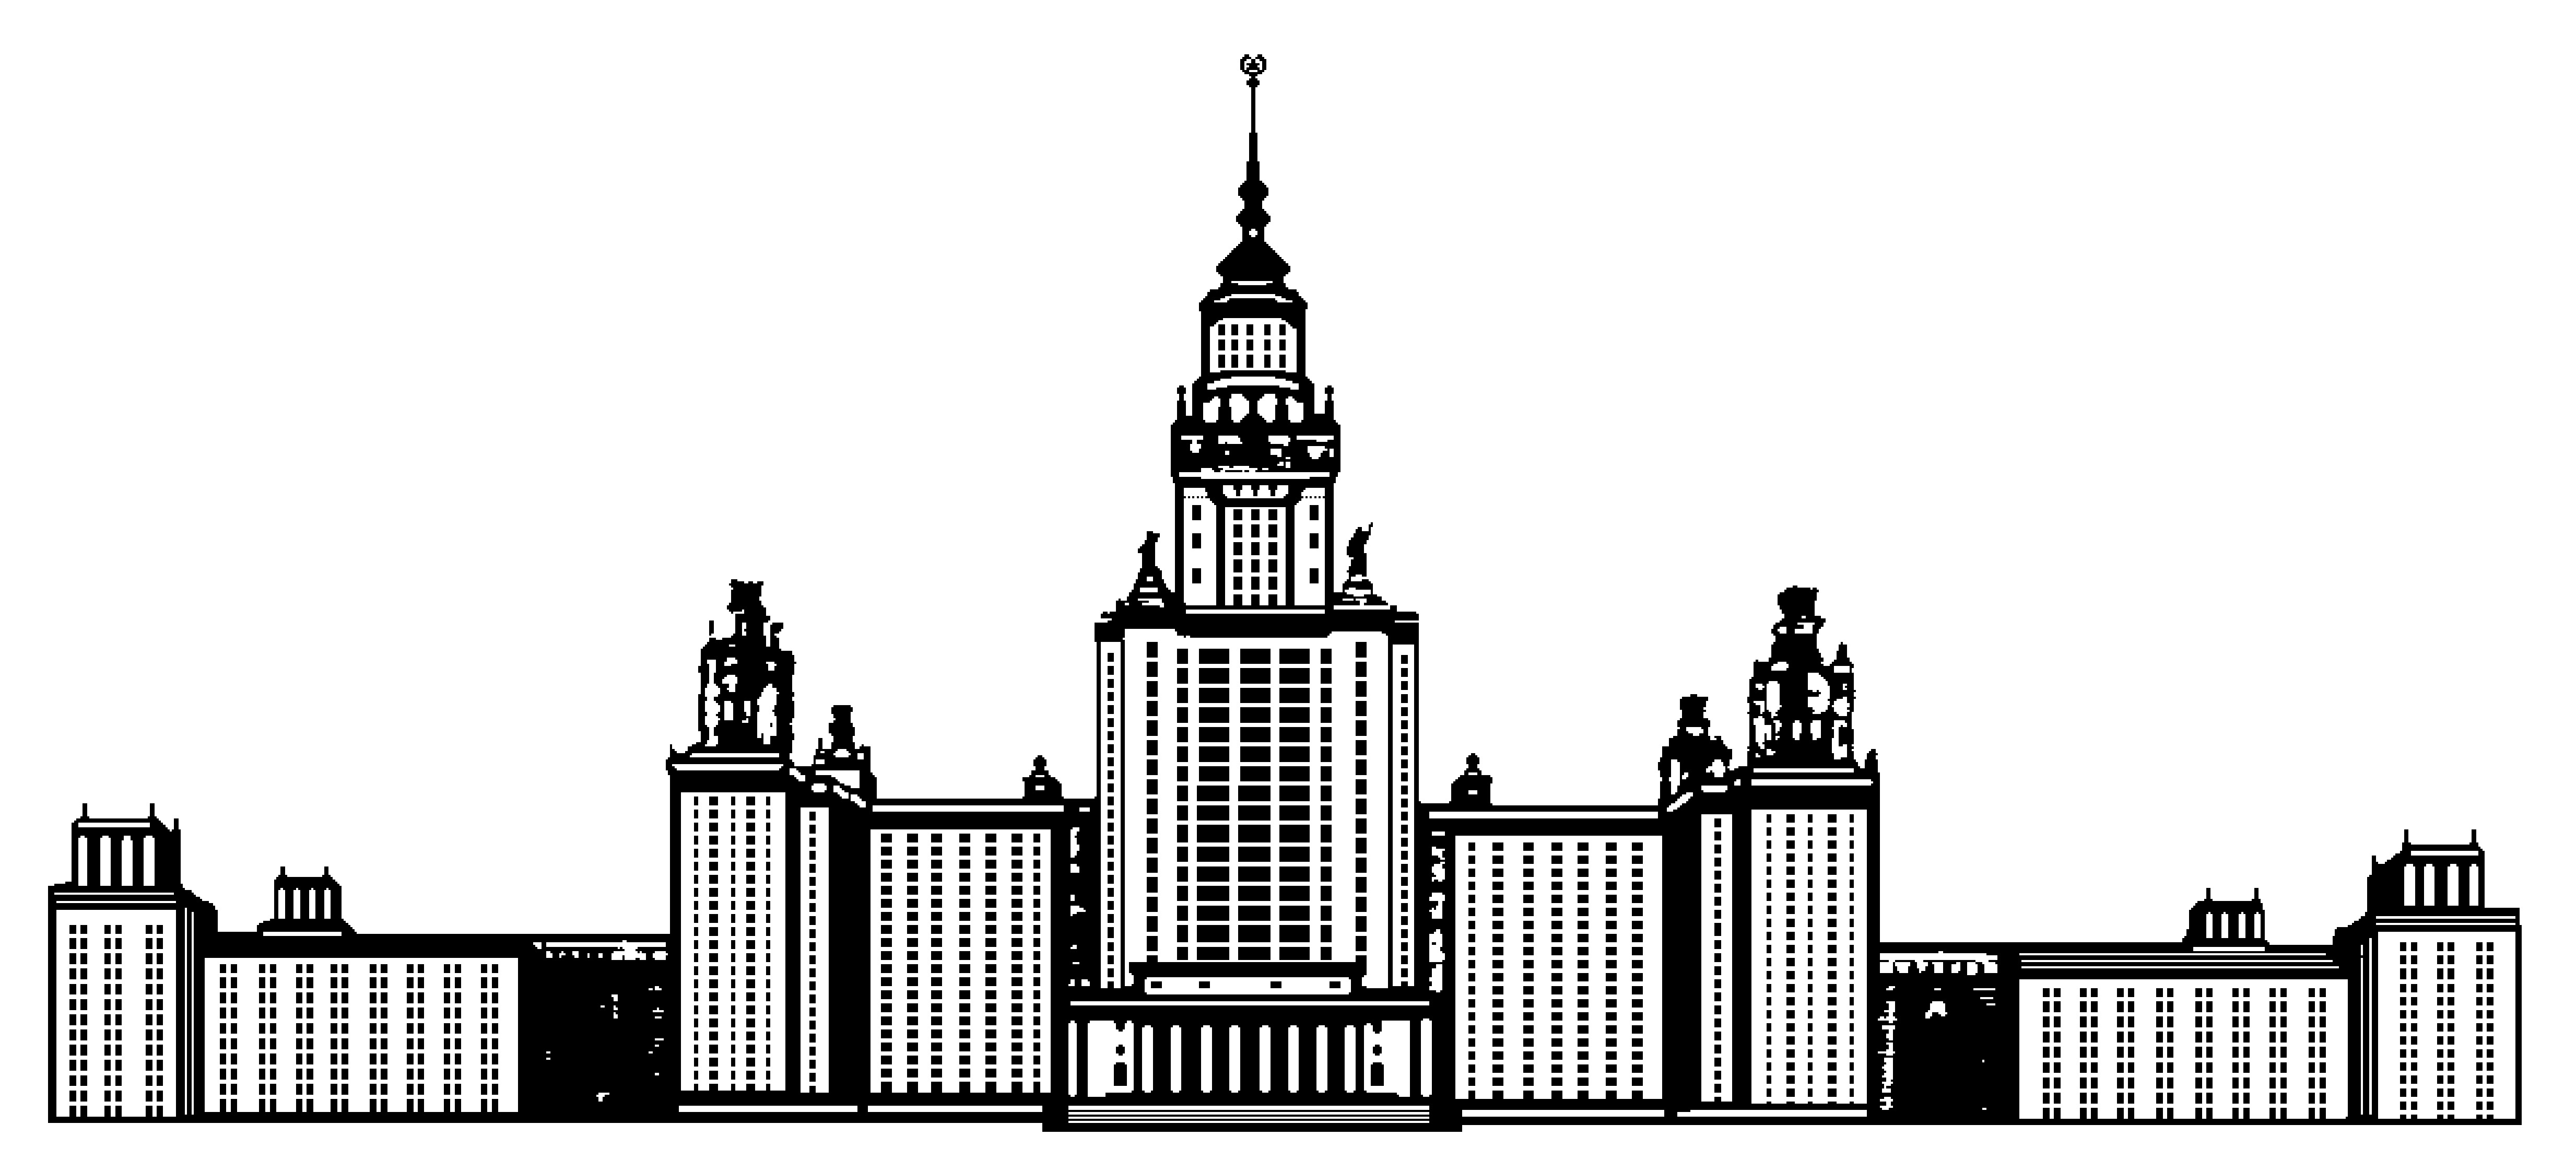
\includegraphics[width=50mm]{./pics/msu.jpg}
        
        \bigbreak
        Факультет Вычислительной Математики и Кибернетики

        Кафедра Математических Методов Прогнозирования

        \vspace{10mm}

        \textbf{\large ЭССЕ СТУДЕНТА 317 ГРУППЫ}

        \vspace{10mm}

        \textbf{\Large <<Свёрточные нейронные сети>>}

        \vspace{10mm}
        
        \begin{flushright}
            \parbox{0.5\textwidth}{
                Выполнил:

                студент 3 курса 317 группы
                
                Сидоров Леонид Станиславович
            }
        \end{flushright}
        \vspace{\fill}
        Москва, 2021   
    \end{center}
\end{titlepage}

\newpage
    \begin{center}
        \textbf{Аннотация}
    \end{center}

    Успехи свёрточных нейронных сетей в области классификации изображений в 2012 году пробудили общественный интерес к сфере глубокого 
    обучения. С тех пор эту архитектуру оттеснили более новые активно развивающиеся алгоритмы и парадигмы, однако наряду с рекуррентными 
    и полносвязными сетями подходы на основе свёртки являются основой машинного обучения, многие принципы из которых повлияли на всю 
    предметную область.

    Именно поэтому в этой работе мы ознакомимся с основными принципами функционирования свёрточных сетей, с их предшественниками и 
    попробуем подумать о будущем этой парадигмы.

    \newpage

    \newpage
        \tableofcontents
    \newpage

    \section{Введение}

    Свёрточная нейронная сеть (\textit{convolutional neural network, CNN}) \cite{LeCun1989}~--- это специальный вид 
    нейронной сети для 
    обработки данных, имеющих сеточную топологию. Примерами могут служить временные ряды, которые можно рассматривать как одномерную 
    сетку измерений, выбираемых через регулярные промежутки времени, а также изображения, рассматриваемые как двумерная сетка пикселей. 
    Свёрточные сети чрезвычайно успешны в практических приложениях. Своё название они получили благодаря использованию математической 
    операции свёртки. Свёртка~--- это линейная операция на паре функций, которую можно интерпретировать как «схожесть» одной 
    функции с отражённой и сдвинутой копией другой. Свёрточные сети – это нейронные сети, в которых вместо общей 
    операции умножения на матрицу, по крайней мере в одном слое, используется свёртка.

    \begin{figure}[ht]
        \centering
        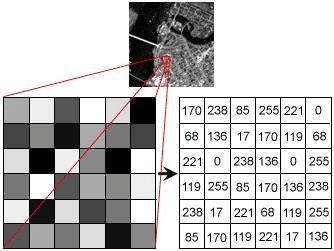
\includegraphics[scale=0.5]{pics/image_representation.png}
        \caption{Монохромное изображение в виде двумерной матрицы \cite{imageRepr}.}
        \label{image_representation}
    \end{figure}

    \subsection{Что такое изображение}

    В последнее время особенным успехом пользуются свёрточные сети, применяемые для классификации изображений. Как уже упоминалось выше, 
    цифровое изображение можно представить в виде сетки пикселей. В случае монохромного изображения эту сетку реализует двумерный 
    массив размера $\hat{H} \times \hat{W}$ ($\hat{H}$ и $\hat{W}$~--- высота и ширина изображения в пикселях соответственно), элементами которого являются 
    значения яркости пикселей из диапазона $[0, 255]$ (Рис. \ref{image_representation}). Случай 
    цветного изображения несколько более сложный, для кодирования цвета могут использоваться различные цветовые схемы, например, \textbf{XYZ}, 
    \textbf{HSV}, или \textbf{YCbCr}, однако самой популярной является схема \textbf{RGB}, в которой цвет пикселя кодируется тремя 
    значениями из диапазона $[0, 255]$, каждое из которых соответствует своему цвету~---  красному, зелёному или синему. 
    В этом случае изображение представляет собой трёхмерный тензор размера $\hat{H} \times \hat{W} \times \hat{C}$, где $\hat{C}$~--- количество цветов 
    (в нашем случае $3$). Этот вариант представления пользуется особой популярностью в сфере обучения свёрточных сетей.

    \subsection{Линейный подход к классификации на несколько классов} \label{linear_section}

    \begin{figure}[ht]
        \centering
        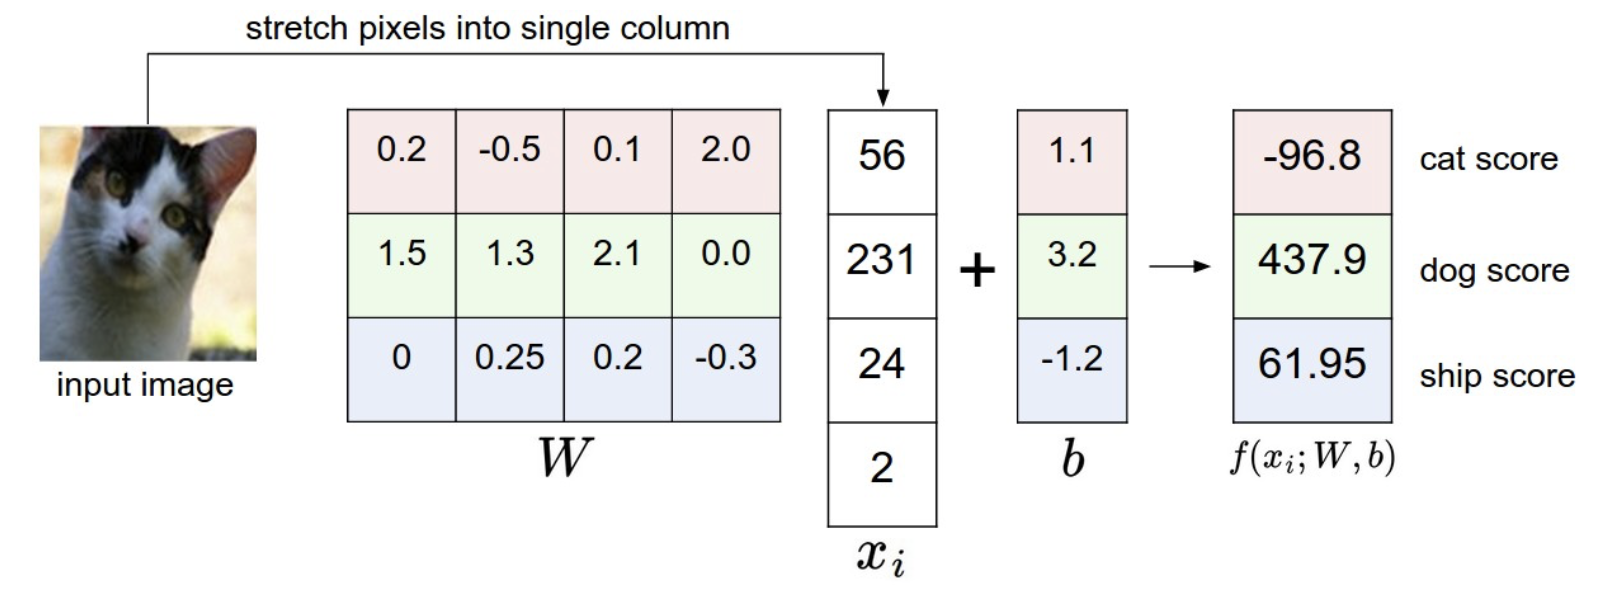
\includegraphics[scale=0.5]{pics/linear_classification.png}
        \caption{Пример работы линейной модели классификации изображений \cite{cs231n}.}
        \label{linear_classification}
    \end{figure}

    Изначально изображения обрабатывались линейными моделями. Приведём пример такого подхода. Допустим, мы решаем задачу 
    классификации изображений, тогда $x_i \in \mathbb{R}^D, i = 1, \dots, N$~--- это обучающая выборка, состоящая из 
    изображений, то есть трёхмерных тензоров, приведённых к виду одномерного вектора размера $D = \hat{H} \times \hat{W} \times \hat{C}$, 
    $N$~--- размер выборки. $y_i \in 1, \dots, K$~--- это метки классов для каждого объекта выборки, где $K$~--- количество классов. 
    Линейная классификатор имеет следующий вид:
    $$f(x_i ,W , b) = W x_i + b,$$ 
    \noindent где $W \in \mathbb{R}^{K \times D}$ и $b\in \mathbb{R}^K$~--- обучаемые параметры. 
    Модель получает на вход вектор длины $D$ а возвращает вектор длины $K$, содержащий оценки для каждого класса. 
    Матрицу $W$ часто называют весами модели, а вектор $b$ смещением, потому 
    что он влияет на выходные оценки, но не взаимодействует с входными данными $x_i$. 
    
    Пример работы алгоритма изображён на Рис. \ref{linear_classification}, изображению присуждается класс с наивысшей оценкой.

    \begin{figure}[ht]
        \centering
        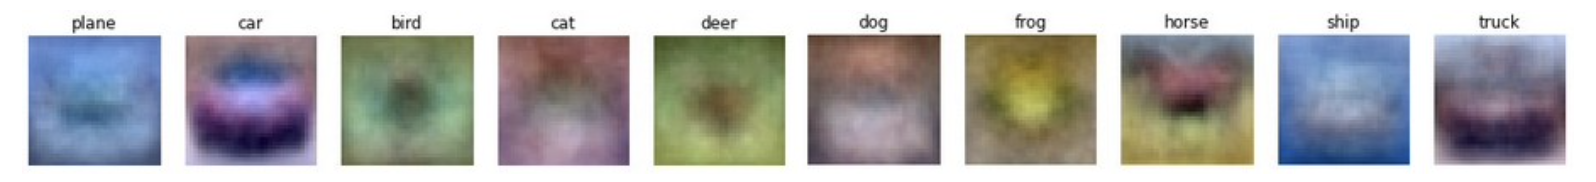
\includegraphics[scale=0.5]{pics/linear_weights.png}
        \caption{Матрица весов обученного линейного классификатора \cite{cs231n}.}
        \label{linear_weights}
    \end{figure}

    Преимуществами такого подхода являются низкая вычислительная сложность и интерпретируемость результатов, на Рис. \ref{linear_weights} 
    изображены веса обученной модели. Как мы видим, они в целом напоминают типичных представителей каждого класса. Поэтому при интерпретации 
    мы просто можем сказать, что входное изображение элементарно "похоже" на один из эталонов. Однако уже на этом изображении мы видим 
    серьёзные недостатки рассмотренного алгоритма, фон у типичных представителей классов "самолёт" и "корабль" является синим, то есть 
    любое синее изображение с большой долей вероятности будет отнесено к одному из этих классов. Помимо этого мы можем заметить, что и ракурс 
    у большинства эталонов является строго заданным, поэтому алгоритм способен распознать автомобиль только с правильного угла. Также 
    линейная модель не учитывает главной особенности изображений~--- взаимосвязь соседних пикселей. 
    
    Эти и многие другие недостатки линейных моделей решают свёрточные нейронные сети, к изучению устройства которых мы и переходим со 
    следующего раздела.

    \section{Устройство свёрточной нейронной сети}

    \subsection{Операция дискретной свёртки}

    Для начала ответим на вопрос, что же такое свёртка. Прообразом операции, используемой в нейронных сетях является линейное преобразование 
    из функционального анализа $(f*g)(t):=\int_{-\infty }^{\infty }f(\tau )g(t-\tau )\,d\tau,$ где $f$ и $g$~--- некоторые функции.

    Его дискретной аппроксимацией является выражение $(f*g)[n]=\sum_mf[m]g[n-m],$ где $f$ и $g$~--- векторы 
    одинаковой длины, а индекс $m$ "пробегает" все их элементы.

    Свёрткой в нейронных сетях называется обобщение этого преобразования на случай векторов разной длины, для начала
    рассмотрим его одномерный случай. Пусть имеется два вектора $A = (a_1,a_2,\dots,a_n)$ и
    $B = (b_1,\dots,b_k)$. Тогда одномерной свёрткой $A$ по $B$ называется вектор $C = (c_{i})^{n - k + 1}$, в котором:
    
    $$c_i = \sum_{j=1}^{k}a_{i + j - 1}b_{j}$$

    $B$ также называется \textbf{ядром} свёртки. Пример такой одномерной свёртки показан на рис. \ref{1d_conv}, где $B=(1,0,-1)$. 
    Как мы видим, такое преобразование изменяет размер исходного вектора. Решить эту проблему можно с помощью добавления отступа к 
    краям исходного изображения, в нашем случае это отступ ширины один, заполненный нулями.
    Однако существуют разные виды отступов:
    \begin{itemize}
        \item нулевой~--- отступ заполняется нулями;
        \item константный~--- отступ заполняется указанной константной величиной;
        \item зеркальный~--- отступ заполняется зеркально относительно края основного вектора;
        \item циклически~--- отступ заполняется элементами с другого края основного вектора.
    \end{itemize}

    В правой части рисунка изображена свёртка с шагом два, её мы рассмотрим в следующих разделах.

    \begin{figure}[ht]
        \centering
        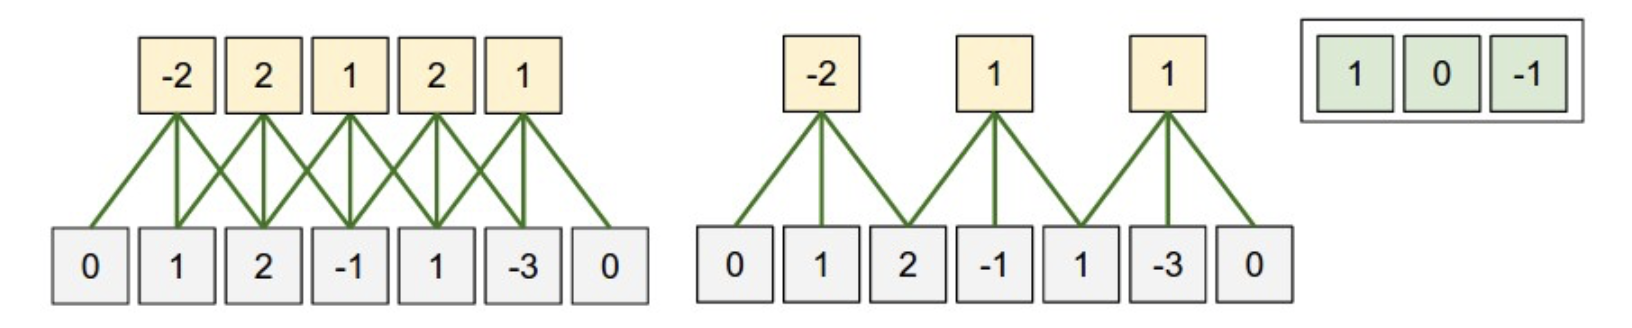
\includegraphics[scale=0.5]{pics/1d_conv.png}
        \caption{Пример использования одномерной свёртки \cite{cs231n}.}
        \label{1d_conv}
    \end{figure}

    Одномерная свёртка распространена в теории сигналов, где она применяется к некоторому временному ряду. 
        
    Аналогичную идею можно применить и к объектам большей размерности, например, к матрицам или
    многомерным тензорам. Размерность ядра, соответственно, тоже будет увеличиваться. 
    
    Для матриц двумерная свёртка определяется следующим образом: пусть $A = (a_{ij})^{n \times m}$ - исходная
    матрица, $K = (k_{ij})^{k \times l}$ - ядро свёртки, тогда двумерной свёрткой матрицы $A$ по
    ядру $K$ будет являться матрица $C=(c_{ij})^{n-k+1 \times m-l+1}$, в которой

    $$C_{ij} = \sum_{x=1}^{k}\sum_{y=1}^{l}A_{i+x-1,j+y-1}K_{xy}.$$

    Пример двумерной свёртки представлен на рис. \ref{2d_conv}.

    \begin{figure}[ht]
        \centering
        \begin{subfigure}[b]{0.5\textwidth}
            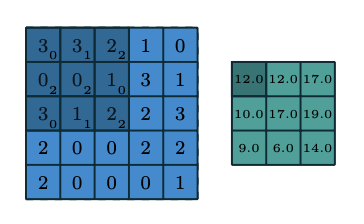
\includegraphics[width=\linewidth]{pics/2d_conv.png}
            \caption{Вычисление одного элемента}
        \end{subfigure}
        \begin{subfigure}[b]{0.2\textwidth}
            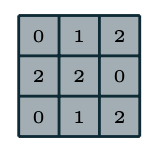
\includegraphics[width=\linewidth]{pics/2d_kernel.png}
            \caption{Ядро свёртки}
        \end{subfigure}
        \caption{Пример использования одномерной свёртки \cite{dumoulin2016guide}.}
        \label{2d_conv}
    \end{figure}

    В компьютерном зрении, используются самые разные виды свёрток. Выбрав определённое ядро, мы можем добиться самых разных результатов, 
    например, размытия изображения, выделения вертикальных или горизонтальных линий, выделения контуров и т.д. .

    \subsection{Свёртка как основная часть структуры свёрточного слоя}

    Мы вплотную подобрались к основному элементу свёрточной нейронной сети~--- свёрточному слою.
    Как известно, все операции, проводимые внутри нейронной сети, осуществляются над тензорами
    большой размерности. Введём в нейронную сеть слой, который будет принимать на вход тензор 
    и применять у нему свёртку с помощью ядра заданного размера. Будем
    рассматривать частный случай~--- трёхмерные тензоры, которыми чаще всего оперируют при
    работе с изображениями. Кроме того, будем рассматривать ядра, которые имеют такую же третью размерность,
    что и входные тензоры ($\hat{C}$~--- количество каналов).
    Математически это записывается следующим образом:
    
    $$ C_{ij} = \sum_{l=1}^{h} \sum_{p=1}^{w} \sum_{k=1}^{c} X_{i+l-1, j+p-1, k} K_{l p k},$$

    \noindent где $X \in \mathbb{R}^{\hat{H} \times \hat{W} \times \hat{C}}$~--- входной тензор, 
    $K \in \mathbb{R}^{h\times w \times \hat{C}}$~--- ядро свёртки,
    $C \in \mathbb{R}^{H-h+1\times W-w+1}$~--- свёртка, $h$ и $w$~--- высота и ширина свёртки соответственно.

    Заметим, что на выходе слоя мы получаем тензор состоящий всего из одного канала. 
    Основная идея свёрточного слоя заключается в использовании нескольких ядер свёртки. 
    Каждому ядру соответствует своё преобразование, например, детектирование контуров изображения 
    или применение некоторого фильтра. Для повышения предсказательной способности алгоритма мы бы 
    хотели иметь доступ сразу к нескольким версиям преобразованного изображения, поэтому использование множества
    различных свёрточных ядер оправдано. На выходе в таком случае мы будем получать тензор, количество каналов которого
    равно количеству используемых в слое ядер свёртки. Пример подобного преобразования представлен на Рис. \ref{conv_channels}.

    \begin{figure}[ht]
        \centering
        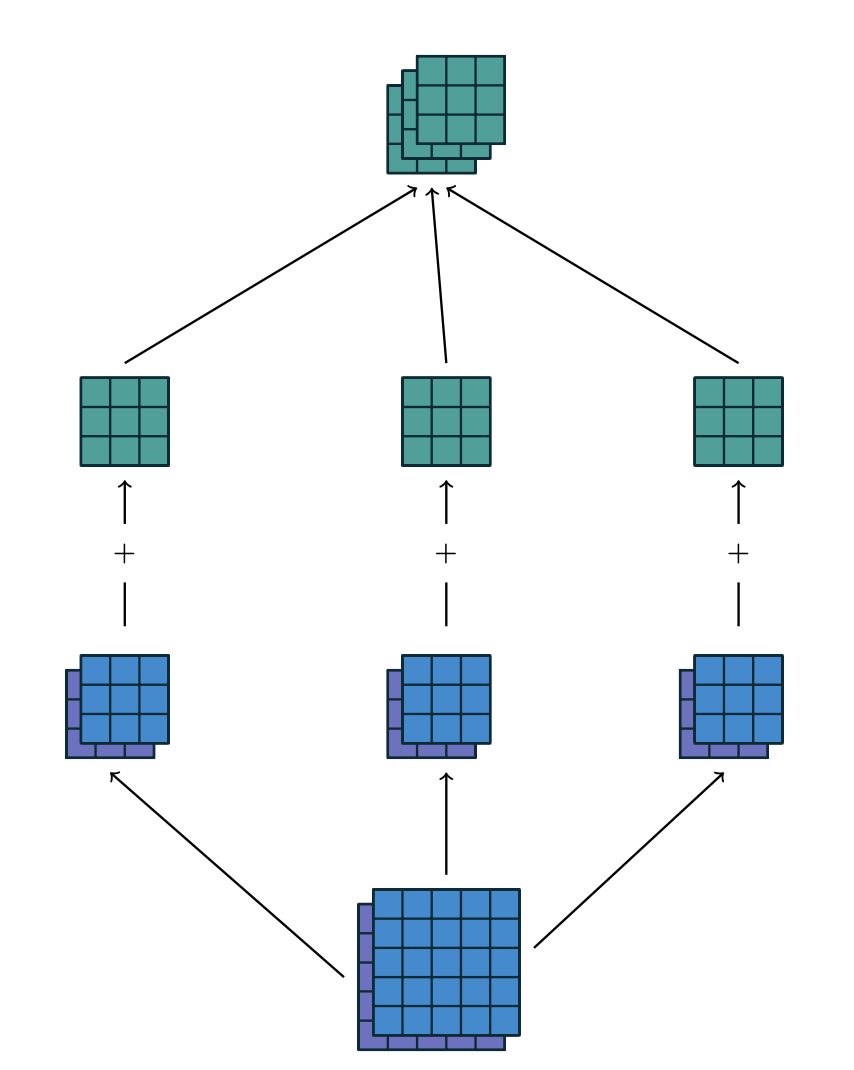
\includegraphics[scale=0.5]{pics/conv_channels.png}
        \caption{Принцип работы свёрточного слоя с несколькими ядрами \cite{dumoulin2016guide}.}
        \label{conv_channels}
    \end{figure}
        
    При рассмотрении одномерного случая мы упомянули, что, варьируя размер отступа, можно сохранять
    первоначальную длину входного вектора. В многомерном случае это правило также выполняется. Если 
    ширину и высоту входного тензора необходимо сохранить, то это также можно сделать с помощью 
    отступа (рис. \ref{conv_mods}a).

    \begin{figure}[ht]
        \centering
        \begin{subfigure}[b]{0.33\textwidth}
            \centering
            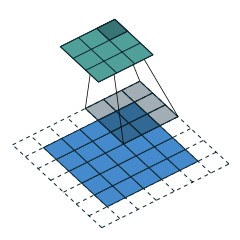
\includegraphics[width=\linewidth]{pics/padding.png}
            \caption{использование отступа}
        \end{subfigure}
        \begin{subfigure}[b]{0.33\textwidth}
            \centering
            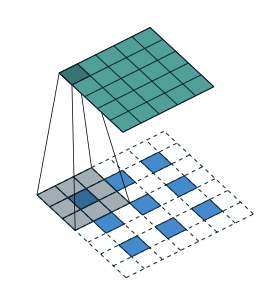
\includegraphics[width=\linewidth]{pics/stride.png}
            \caption{шаг наложения свёртки}
        \end{subfigure}
        \begin{subfigure}[b]{0.33\textwidth}
            \centering
            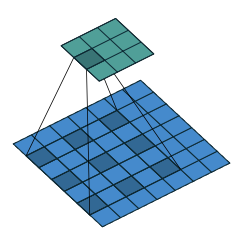
\includegraphics[width=\linewidth]{pics/dilation.png}
            \caption{расширение области зависимости}
        \end{subfigure}
        \caption{Примеры модификаций операции свёртки \cite{dumoulin2016guide}.}
        \label{conv_mods}
    \end{figure}

    Ещё одна опция~--- это значительное понижение размерности, выбирая шаг, с которым будет перемешаться
    окно свёртки (Рис. \ref{conv_mods}b), можно кратно уменьшить размер входного
    тензора. То есть движения этого окна осуществлять не на соседние клетки, а через одну или
    даже несколько.
        
    Мы можем сказать, что свёртки собирают информацию с некоторой области, которую можно
    по-разному интерпретировать в зависимости от вида ядра, например, судить,
    есть ли в данном фрагменте изображения вертикальные линии. В качестве
    ещё одной модификации процесса свёртки предлагается расширение области действия ядра, но
    не за счёт фактического увеличения размера ядра, а за счёт увеличения покрываемой области 
    (Рис. \ref{conv_mods}c). Элементы, с которых берутся значения, не расположены по
    соседству, а удалены друг от друга на некоторую одинаковую для всех величину.
        
    Все эти базовые приёмы манипуляции с ядром свёртки позволяют нам проводить гибкую настройку
    структуры нейронной сети в целом. Но на этом рассмотрение свёрточного слоя не заканчивается, помимо
    процесса свёртки в него входят этапы нелинейного преобразования признаков и их агрегации.
    Эти преобразования мы рассмотрим в следующих разделах.

    \subsection{Свёртка как линейная операция}

    Но перед этим отметим, что применение свёртки в нейронной сети всё ещё остаётся линейной операцией.

    Возьмем для примера свертку c $3 \times 3$ ядром, применённую к $4 \times 4$ изображению (все остальные параметры стандартные). 
    Если бы вход и выход были развернуты в 
    векторы (слева направо, сверху вниз), свертка могла бы быть представлена в виде разреженной матрицы $C$, где ненулевыми 
    элементами являются элементы $w_{i,j}$ ядра (причем $i$ и $j$ являются строкой и столбцом ядра соответственно). Матрица $C$ 
    представлена на Рис. \ref{linear_conv}.

    \begin{figure}[ht]
        \centering
        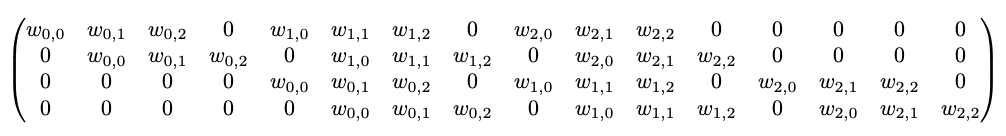
\includegraphics[scale=0.8]{pics/linear_conv.png}
        \caption{Свёртка в виде матрицы, размер ядра $3 \times 3$, а изображения $4 \times 4$ \cite{dumoulin2016guide}.}
        \label{linear_conv}
    \end{figure}

    Эта линейная операция принимает матрицу, представленную в виде $16$-мерного вектора, а возвращает 
    $4$-мерный вектор, который позже преобразуется в выход размера $2 \times 2$.

    Используя это представление, обратный проход легко получается путем транспонирования $C$. То есть, как и в случае линейного слоя, 
    градиент пропускается путем его умножения на $C^T$. Эта операция принимает $4$-мерный вектор в 
    качестве входа и возвращает $16$-мерный вектор в качестве выхода, его шаблон связности совместим с $C$ по построению.

    Примечательно, что ядро $w$ определяет как $C$, так и $C^T$, используемые для прямого и обратного проходов.

    Также отметим, что если поменять $C$ и $C^T$ местами (то есть прямой и обратный проходы), то мы получим операцию 
    обратной свёртки (\textit{deconvolution}), которая применяется, например, в моделях сегментации. Однако эта 
    операция, применённая непосредственно после свёртки, не гарантирует восстановления исходных данных, потому что свёртка является 
    необратимым преобразованием, сохраняется лишь форма исходного тензора ($\hat{H}$ и $\hat{W}$).
        
    \subsection{Нелинейность и пулинг}

    \begin{figure}[ht]
        \centering
        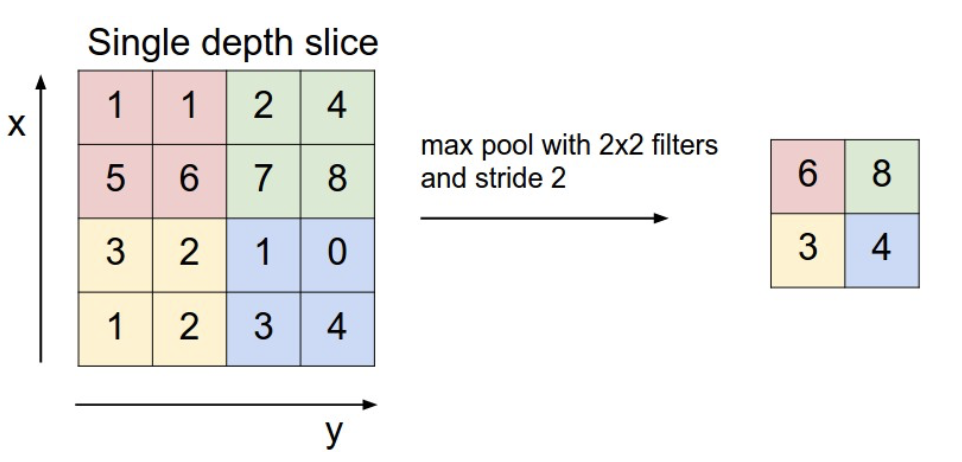
\includegraphics[scale=0.5]{pics/maxpooling.png}
        \caption{Пример пулинга~--- взятие максимума, или \textit{MaxPool} \cite{cs231n}.}
        \label{maxpooling}
    \end{figure}

    Важной частью свёрточного слоя является процесс преобразования и фильтрации полученных
    признаков. Процесс свёртки заканчивается передачей сформированного тензора признаков, его
    необходимо обработать, пропустив через нелинейные функции активации. Выбор нужной
    функции очень сильно влияет на функционал нейронной сети. Варьируя разные функции активации,
    можно добиваться разных результатов. Укажем наиболее популярные функции:

    \begin{itemize}
        \item ReLu: $f(x) = \max(0, x)$;
        \item Сигмоида: $f(x) = \frac{1}{1 + e^{-x}}$;
        \item Гиперболический тангенс: $f(x) = \frac{e^{2x} - 1}{e^{2x} + 1}$.
    \end{itemize}

    Следующим и последним этапом свёрточного слоя будет процесс понижения размерности, 
    пулинг. Его основная задача заключается в уменьшении размера тензора (а именно $\hat{H}$ и $\hat{W}$), 
    чтобы следующие слои свёрток оперировали над большей областью (генерировали более абстрактные признаки). 
    Для этого входной блок делится на части, над каждой из которых выполняется некоторая операция агрегации, 
    чаще всего это взятие максимума или среднего (Рис. \ref{maxpooling}).

    Однако на этом виды пулинга не заканчиваются. Они могут отличаться друг от друга как видом
    функции агрегации ($L_2$-норма, выбор значения с некоторой вероятностью), так и формой входа или 
    выхода (выбор $k$ максимальных элементов). Например, в динамическом пулинге размер областей, 
    на которые делится изображение, может быть разным (Рис. \ref{pooling_types}).

    \begin{figure}[ht]
        \centering
        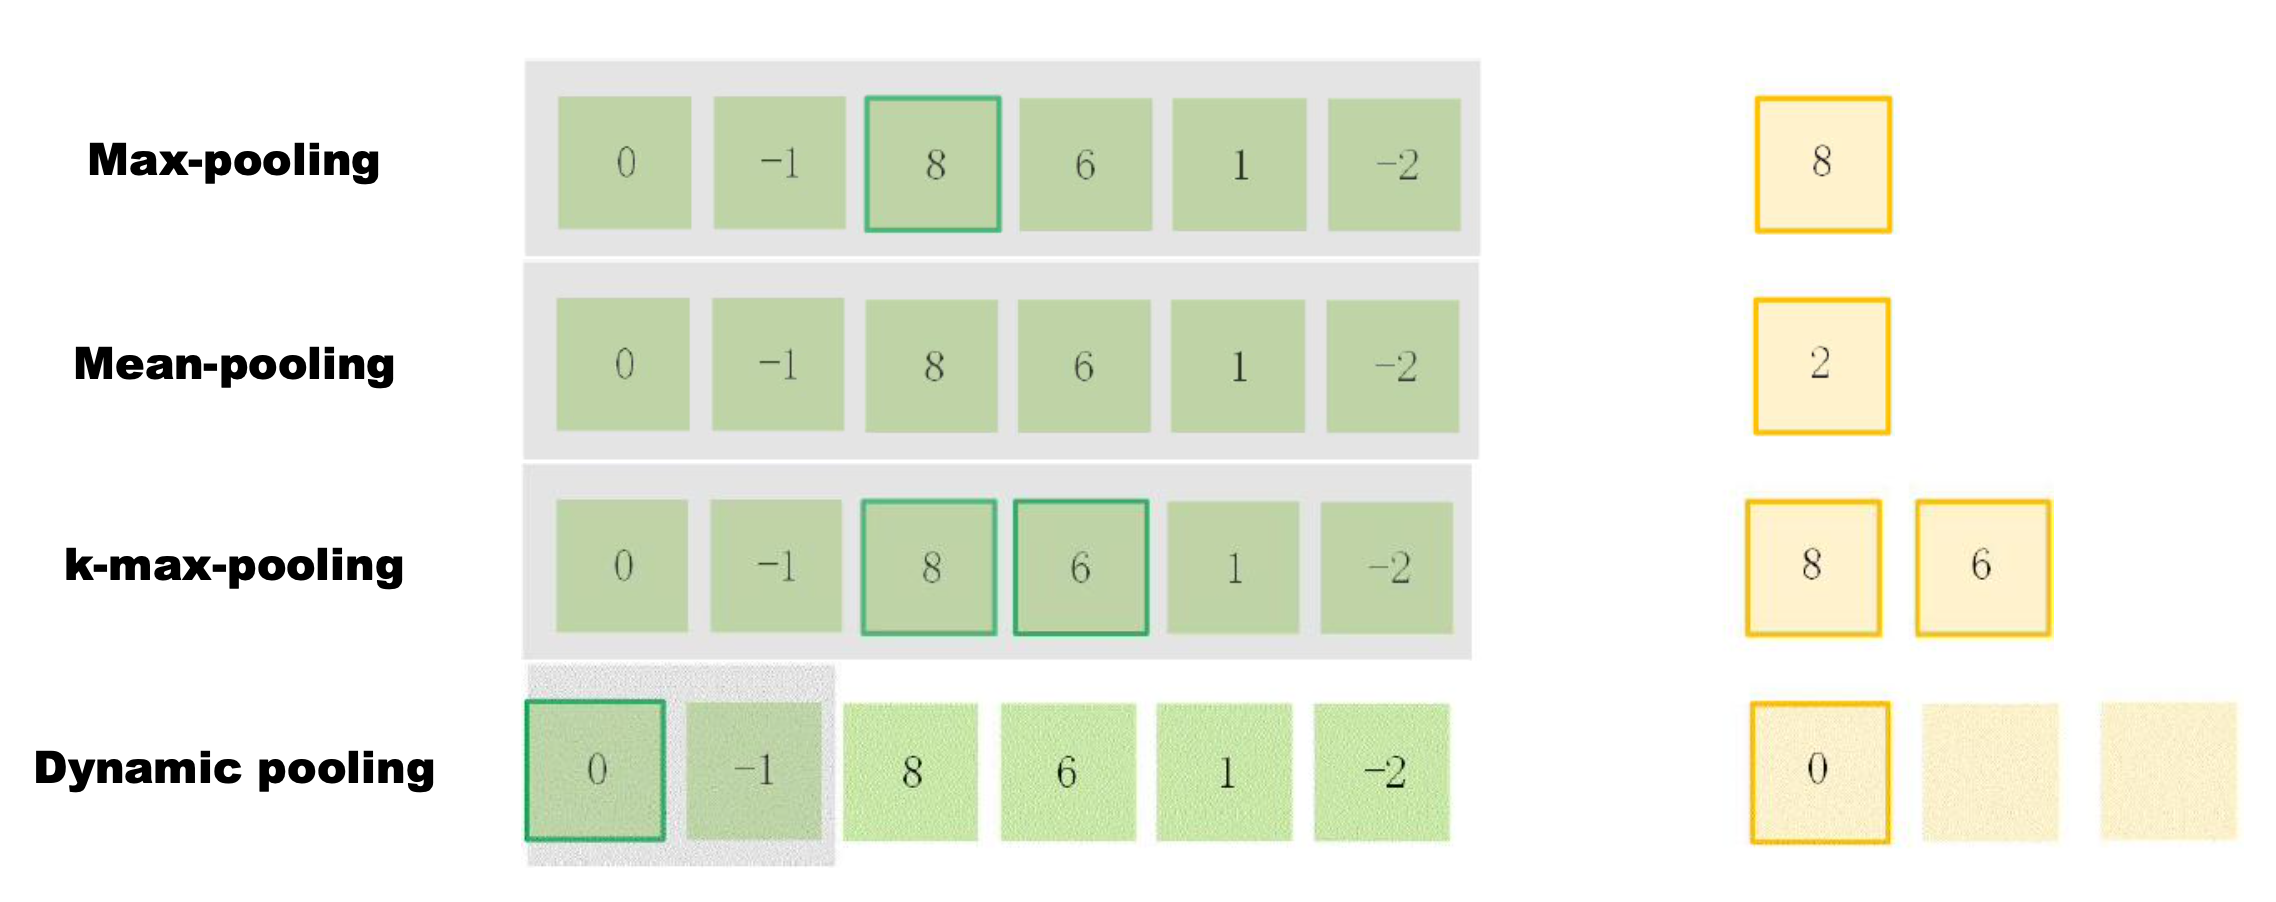
\includegraphics[scale=0.35]{pics/pooling_types.png}
        \caption{Примеры разных видов пулинга \cite{pooling_pic}.}
        \label{pooling_types}
    \end{figure}

    Этот процесс, помимо уменьшения размера тензора, позволяет добавить инвариантность
    представлению изображения к небольшим поворотам или сдвигам, ускоряет вычисления и 
    привносит в сеть дополнительную нелинейность. 
    
    Заметим,
    что здесь нет параметров, по которым бы вычислялся градиент. Во время обратного распространения 
    ошибки градиент передаётся только по тем ячейкам, которые были задействованы при вычислении 
    результата (в случае максимума это только максимальный элемент).

    \subsection{Полносвязный слой}

    Полносвязный слой в свёрточной нейронной сети фактически повторяет устройство линейной модели 
    многоклассовой классификации, рассмотренной в разделе \ref{linear_section}. Только на этот раз 
    модель делает предсказания не на основе значения пикселей изображения, а опираясь на высокоуровневые 
    признаки, полученные после применения нескольких свёрточных слоёв. Поэтому эти предсказания зачастую 
    инвариантны к сдвигу и повороту изображения, а также лишены многих других недостатков линейных 
    классификаторов.

    Добавим, что в случае полносвязного слоя размерность выхода не ограничена количеством классов или 
    какими-либо ещё свойствами задачи. Выход этого слоя может передаваться на следующий, вообще говоря, 
    не финальный слой сети (например, как на Рис. \ref{vgg_axample}).

    Однако полносвязный слой вовсе не обязан присутствовать в свёрточной сети, например, в \cite{he2016deep} 
    он заменён на усреднение по всем элементам тензора (\textit{average pooling}).

    \subsection{Свёртка \texorpdfstring{$1 \times 1$}{1x1}} \label{1x1_sec}

    Отдельного рассмотрения заслуживает свёртка с размером ядра $1 \times 1$, которая является 
    основой многих других подходов в построении свёрточных нейронных сетей.

    Впервые представленный в \cite{lin2013network}, 
    слой свёртки $1 \times 1$ использовался для "сквозного уменьшения количества каналов" или 
    объединения перекрестных каналов. Другими словами, свёртка $1 \times 1$ используется для уменьшения 
    количества каналов при введении нелинейности (Рис. \ref{conv_1x1}).

    \begin{figure}[ht]
        \centering
        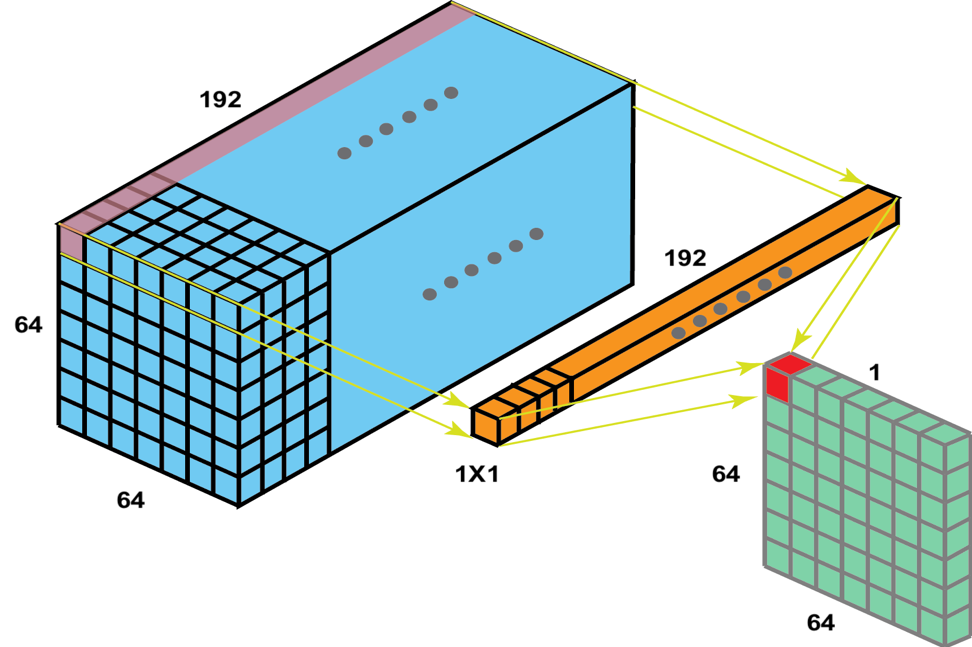
\includegraphics[scale=0.3]{pics/conv_1x1.png}
        \caption{Пример работы $1 \times 1$ свёртки \cite{1x1_conv}.}
        \label{conv_1x1}
    \end{figure}

    Этот трюк особенно полезен при построении глубоких и очень глубоких сетей, многие 
    знаменитые архитектуры использовали его для сокращения количества вычислений 
    \cite{he2016deep, szegedy2015going, iandola2016squeezenet}. Дело в том, что 
    при применении свёртки к слишком глубокому тензору (например, $\hat{C} = 256$), 
    мы можем предварительно уменьшить его глубину с помощью свёртки $1 \times 1$. 
    Таким образом мы можем сохранить глубину самой сети, при этом на порядки уменьшая количество 
    обучаемых параметров.

    Отметим, что $1 \times 1$ свёртка вместе с некоторой нелинейностью фактически образуют 
    нейронную сеть, принимающую на вход сквозные проекции элементов тензора ("столбцы" размера 
    $1 \times 1 \times \hat{C}$). Отсюда происходит и название оригинальной статьи \cite{lin2013network}~--- 
    "Сеть в сети" (\textit{Network in network}).
        
    \subsection{Разреженная связность}

    В слоях традиционной нейронной сети применяется умножение на матрицу параметров, 
    в которой взаимодействие между каждым входным и каждым выходным элементами описывается отдельным параметром. 
    Это означает, что каждый выходной элемент взаимодействует с каждым входным элементом. В свёрточных сетях же взаимодействия обычно 
    разреженные (это свойство называют ещё разреженной связностью). Визуальное сравнение представлено на Рис. \ref{sparse_interactions}.

    \begin{figure}[ht]
        \centering
        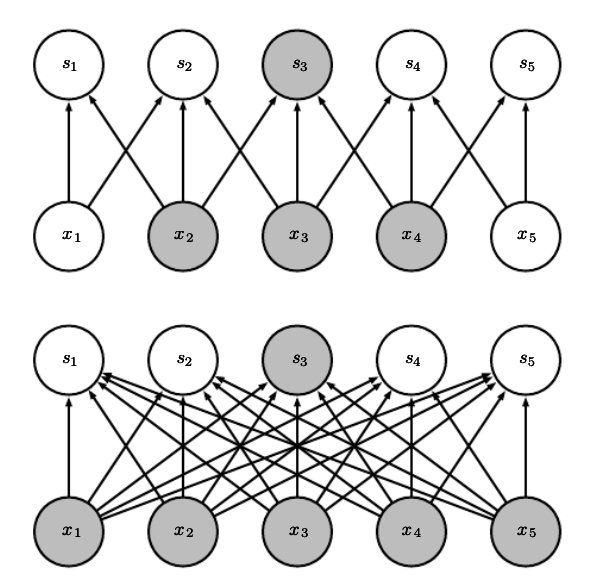
\includegraphics[scale=0.5]{pics/sparse_interactions.png}
        \caption{Сравнение количества параметров для линейного и свёрточного слоёв \cite{Goodfellow-et-al-2016}.}
        \label{sparse_interactions}
    \end{figure}
    
    Это достигается за счет того, что ядро свёртки 
    меньше её входа. Например, входное изображение может состоять из тысяч или миллионов пикселей, однако мы можем 
    обнаружить небольшие значимые признаки, такие как границы, с помощью ядер свёртки, которые занимают 
    только десятки или сотни пикселей. Это значит, что мы можем хранить значительно меньше параметров 
    (достаточно хранить все ядра свёртки), что одновременно снижает 
    требования по памяти модели и повышает ее статистическую эффективность. Кроме того, вычисление выхода 
    требует меньшего количества операций. Вместе все перечисленные улучшения намного повышают эффективность модели.

    \subsection{Организация свёрточной нейронной сети}

    Опишем наиболее распространённую архитектуру свёрточной нейронной сети. На первых уровнях используется
    несколько слоёв свёртки, когда же размеры тензоров становятся достаточно малы (здесь это $\hat{H}$ и $\hat{W}$), 
    их значения агрегируются, например, с помощью полносвязных слоёв. Пример
    подобной сети можно увидеть в \cite{simonyan2014very}, эта архитектура изображена на Рис. \ref{vgg_axample}.

    \begin{figure}[ht]
        \centering
        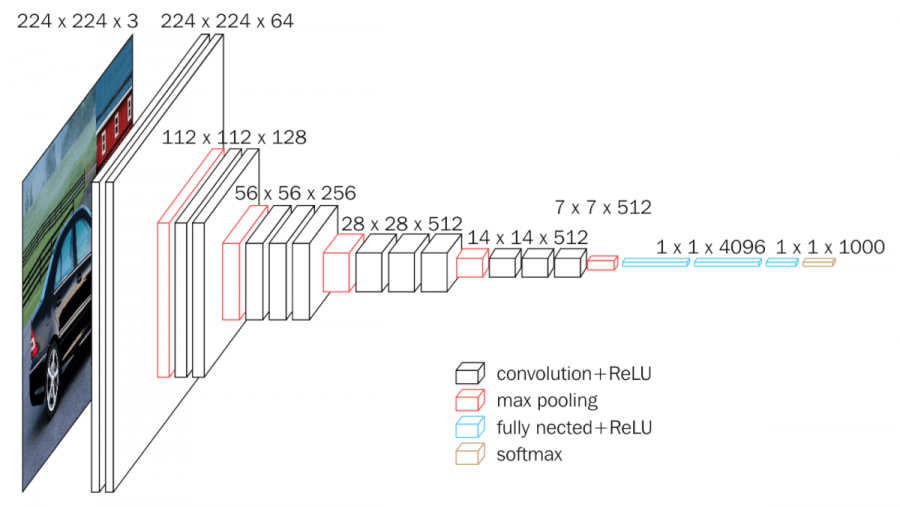
\includegraphics[scale=0.5]{pics/vgg_example.png}
        \caption{Пример архитектуры свёрточной нейронной сети (\textit{VGG16}) \cite{vgg_pic}.}
        \label{vgg_axample}
    \end{figure}

    Выбор элементов ядер остаётся за нейросетью, в процессе обучения, например, с помощью метода обратного 
    распространения ошибки нейросеть сама подбирает нужные значения элементов ядер свёртки с целью 
    минимизации выбранного функционала ошибки.

    Отметим, что свёрточный слой переводит тензор в тензор, обычно размер выхода отличается от размера входа. 
    На практике используют большое количество свёрточных слоёв. С каждым новым
    слоём высота $\hat{H}$ и ширина $\hat{W}$ понижаются, но увеличивается количество каналов $\hat{C}$.
    Для чего это делается, мы опишем в следующем пункте.
        
    \subsection{Смысловая интерпретация свёрточных сетей} \label{cnn_vis}

    Как было упомянуто ранее, различные ядра могут выполнять различные функции,
    например, в двумерном случае ядра могут размывать изображения или выявлять,
    есть ли в области изображения особые структуры, такие как прямые линии, и т.д. . При
    использовании свёрток информация собирается не со всего объекта целиком, а ограниченными 
    участками. Размер каждого такого участка характеризуется размером и
    способом наложения ядра этой свёртки. 
    
    Соответственно, в каждой свёртке обученной нейронной сети 
    хранится конкретная информация об областях изображения (если мы работаем изначально с изображением).
    Повторив операцию свёртки, мы получим уже более высокоуровневое представление
    изображения. То есть, если первая свёртка несла в себе информацию о расположении
    прямых линий, то вторая уже будет содержать информацию об изогнутых.
    Повторяя процесс свёртки многократно, мы будем получать сведения о все
    более сложных абстракциях. Процесс свёртки помогает перейти от конкретных
    деталей к более абстрактным. На последнем шаге мы будем получать высокоуровневые
    представления. Например, от вопроса, есть ли на изображении вертикальные линии, постепенно 
    мы перейдём к вопросу, есть ли на изображении машина или медведь. Визуализация
    иерархии признаков показана на Рис. \ref{conv_vis}.

    \begin{figure}[ht]
        \centering
        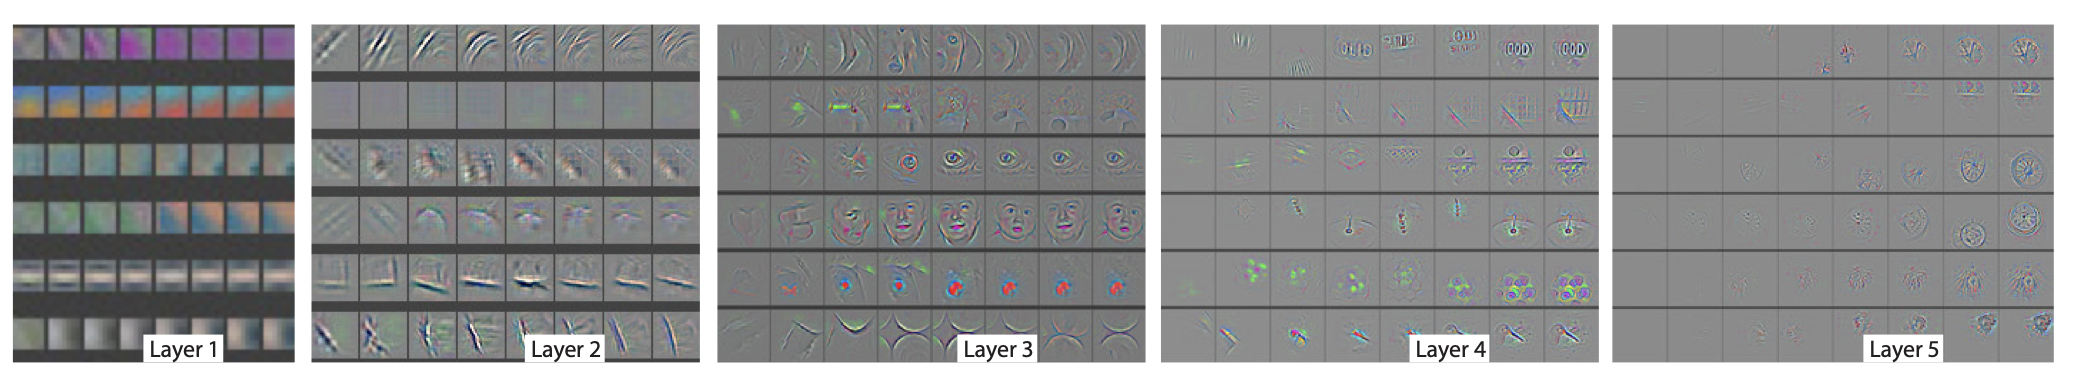
\includegraphics[scale=0.43]{pics/conv_vis.png}
        \caption{Визуализация признаков на различных слоях свёрточной сети (для каждого слоя подвыборка признаков выбиралась случайно, в каждом слое показана эволюция признака по мере обучения)\cite{zeiler2014visualizing}.}
        \label{conv_vis}
    \end{figure}
        
    Немаловажным процессом является пулинг. Его польза обусловлена тем, что
    он уменьшает размеры тензоров, с которым ведутся операции, и процесс
    уменьшения размера происходит на каждом канале независимо друг от друга.

    Отметим ещё одну важную мысль: использование, например, \textit{MaxPooling}
    идейно меняет принцип работы нейросети. Эта операция 
    выбирает из некоторой области максимальное значение, тем самым акцентирует внимание не
    на расположении какого-либо объекта на изображении, а на самом факте наличия
    этого объекта. В итоге мы получаем информацию о содержании изображения.
        
    \subsection{Ещё немного о свёртках}

    В предыдущих разделах были описаны основные принципы, на которые опираются свёрточные нейронные сети. 
    В этой же части мы рассмотрим популярные модификации свёрток:
    
    \begin{enumerate}
        \item \textbf{Пространственные свёртки (Spatial Separable Convolutions)}\\
        Основная идея заключается в представлении исходного ядра в виде произведения 
        двух векторов (Рис. \ref{sep_conv}). В этом случае мы будем применять две свёртки вместо одной, 
        но это значительно сократит количество обучаемых параметров ($6$ против $9$ в случае $3 \times 3$ ядра). 
        Отсюда следует и название метода, каждый вектор соответствует размерностям 
        $\hat{H}$ и $\hat{W}$. Важнейшим недостатком этого метода является 
        ограниченность класса матриц, представимых подобным образом.

        \begin{figure}[ht]
            \centering
            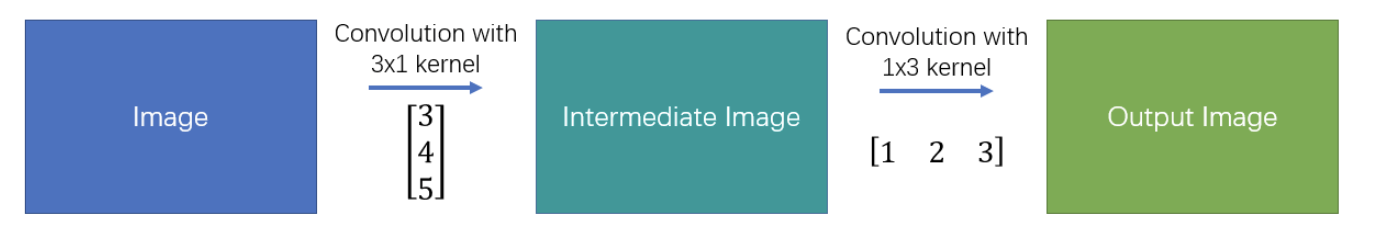
\includegraphics[scale=0.6]{pics/sep_conv.png}
            \caption{Пример применения пространственной свёртки размера $3 \times 3$ \cite{sep_conv}.}
            \label{sep_conv}
        \end{figure}

        \item \textbf{Свёртка с разделением на группы (Group Convolutions)}\\
        Главной идеей этого метода является разделение входного тензора
        на несколько частей, каждая из которых обрабатывается отдельным ядром, 
        после чего результаты конкатенируются (Рис. \ref{conv_group}). В такой 
        свёртке тоже меньше параметров, чем в "полной", однако класс описываемых 
        преобразований значительно больше, чем в предыдущем примере.

        \begin{figure}[ht]
            \centering
            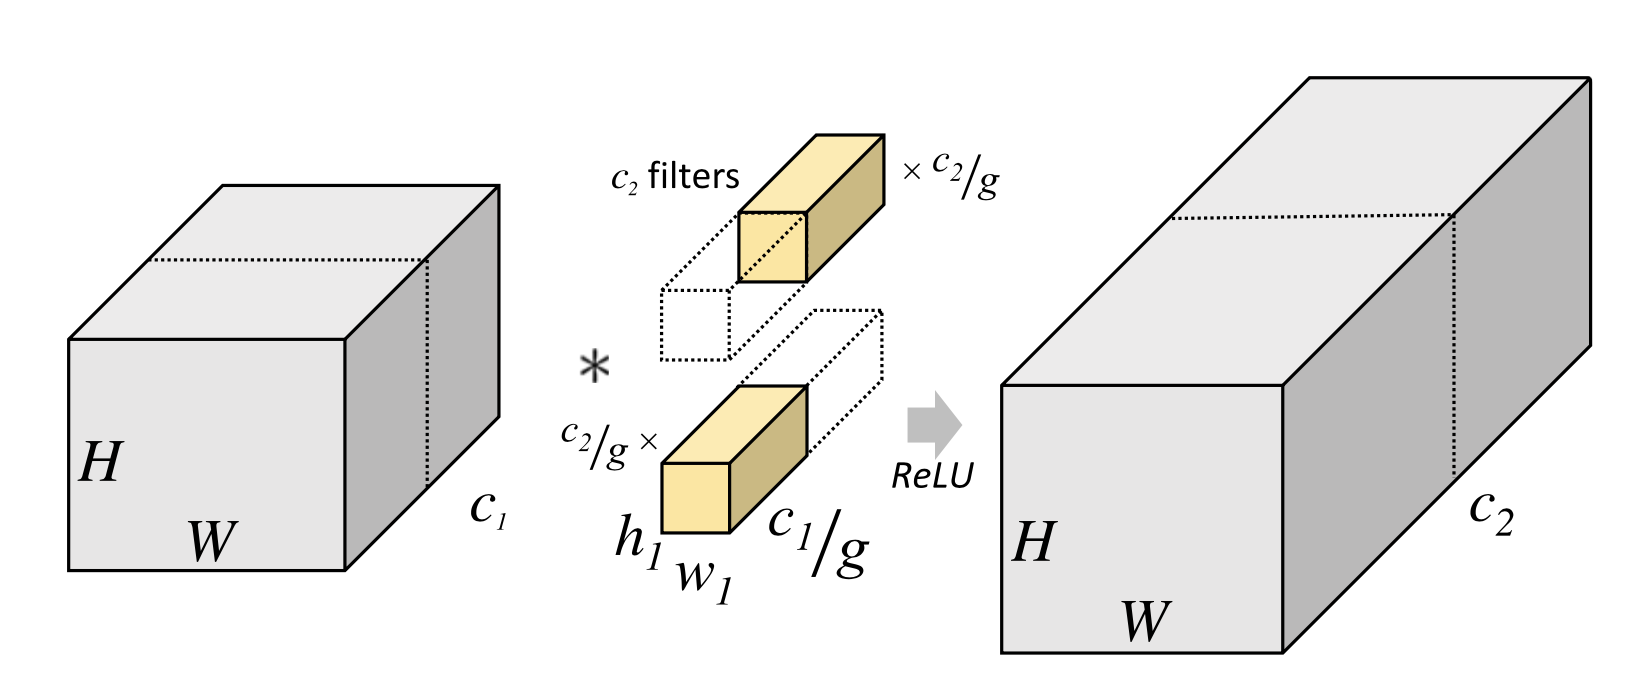
\includegraphics[scale=0.3]{pics/conv_group.png}
            \caption{свёртка с разделением на группы \cite{group_conv}.}
            \label{conv_group}
        \end{figure}
        
        \item \textbf{Свёртка по каналам (Depth-wise Convolution)}\\
        В этом методе тензор делится на каналы, каждый из которых будет 
        обрабатываться своим ядром независимо от других. В таком случае требуется число
        ядер, кратное числу каналов входного тензора. Полученные свёртки конкатенируются, 
        образуя выходной тензор. Свёртка по каналам 
        является частным случаем групповой свёртки, в котором "экономия" 
        параметров максимальна (Рис. \ref{depthwise_conv}a).
            
        \item \textbf{Свёртка по каналам с объединением (Depth-wise Separable Convolution)}\\
        Является модификацией предыдущего метода, к выходу свёртки по каналам
        применяется свёртка $1 \times 1$ (Рис. \ref{depthwise_conv}b) 
        (причины применения свёртки $1 \times 1$ описывались в разделе \ref{1x1_sec}). 

        \begin{figure}[ht]
            \centering
            \begin{subfigure}[b]{0.45\textwidth}
                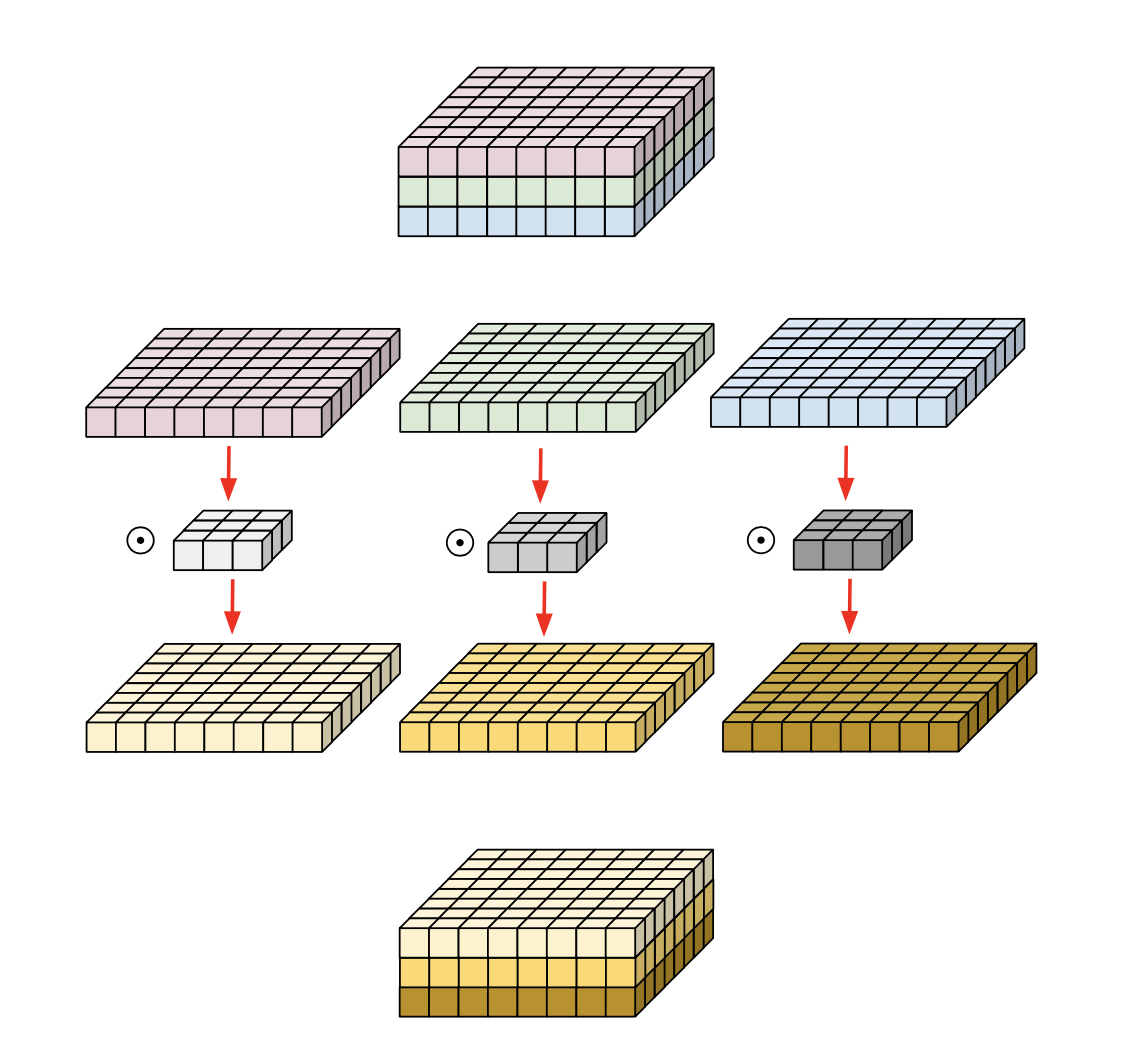
\includegraphics[width=0.7\linewidth]{pics/depth_conv.png}
                \vspace{2.0cm}
                \caption{свёртка по каналам}
            \end{subfigure}
            \begin{subfigure}[b]{0.45\textwidth}
                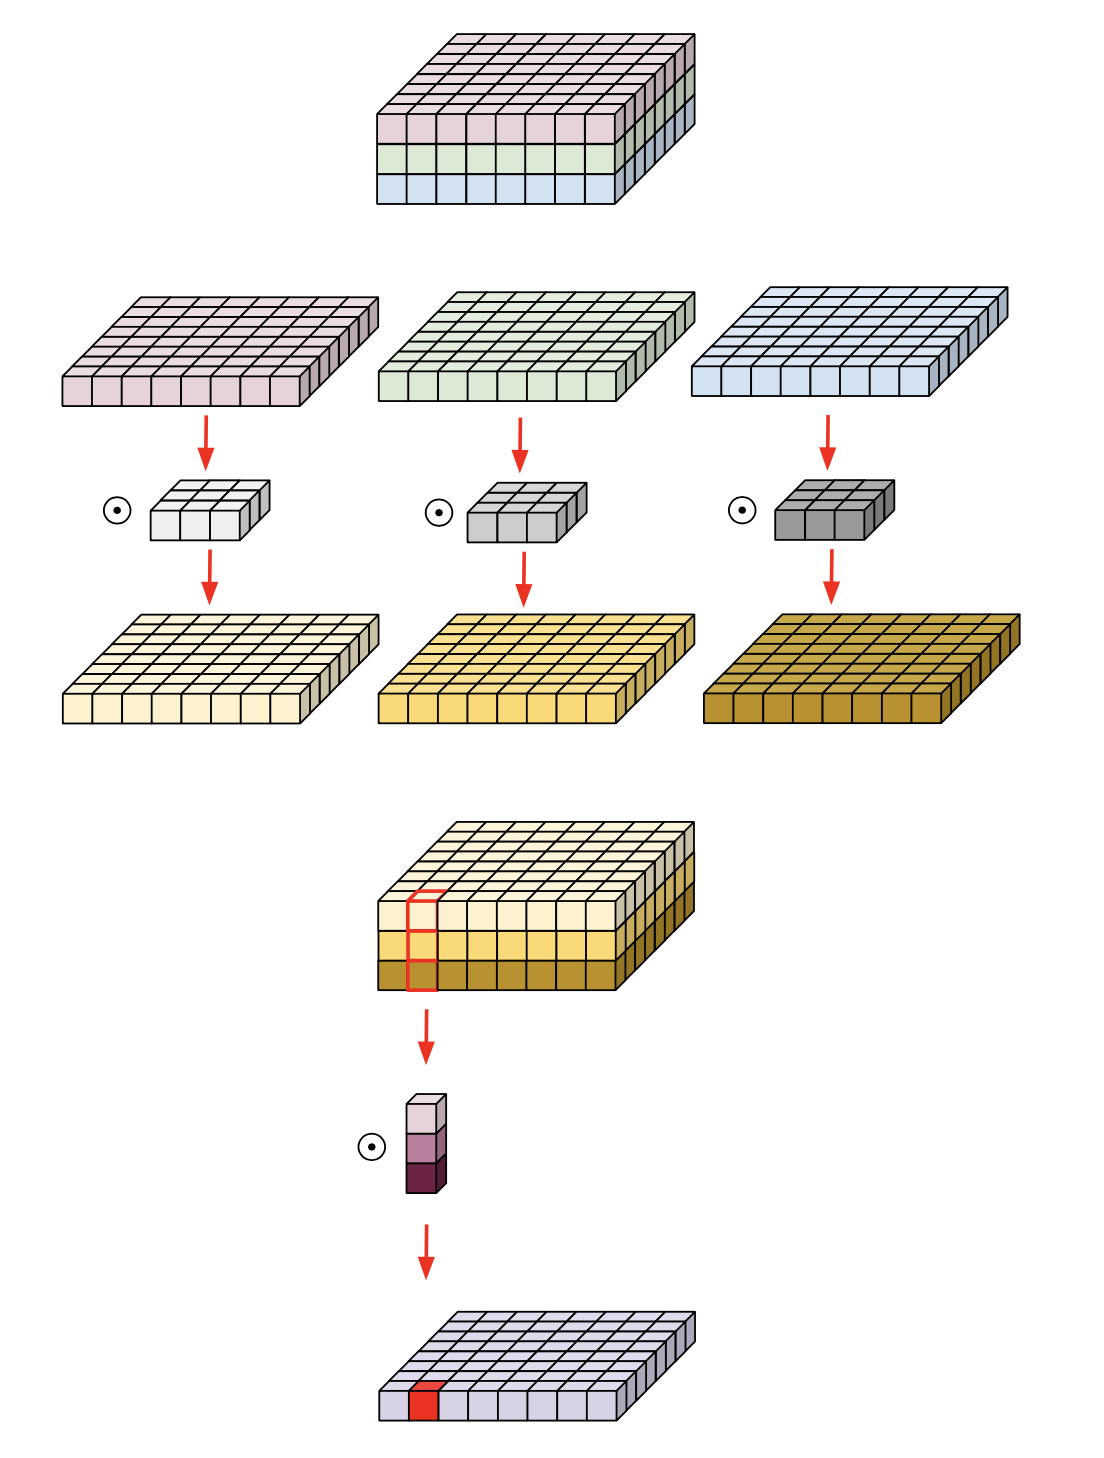
\includegraphics[width=0.7\linewidth]{pics/depth_sep_conv.png}
                \caption{свёртка по каналам с объединением}
            \end{subfigure}
            \caption{Частные случаи групповой свёртки \cite{depthwise_conv}}
            \label{depthwise_conv}
        \end{figure}

    \end{enumerate}

    Мы рассмотрели наиболее популярные модификации свёрток. Комбинируя описанные выше подходы,
    можно придумать огромное количество новых методов, подходящих под каждую конкретную задачу.

    \section{Свёрточные нейронные сети сегодня}

    \subsection{Недостатки свёрточных сетей}

    Теперь поговорим о последних тенденциях в области свёрточных нейронных сетей. Джеффри Хинтон, человек стоящий у 
    истоков глубокого обучения и соавтор сети \textbf{AlexNet} \cite{krizhevsky2012imagenet}, положившей начало 
    буму нейронных сетей в 2012 году, на своём недавнем выступлении \cite{cnn_uncool} заявил, что свёрточные нейронные 
    сети недостаточно хороши для распознавания изображений.

    Он полагает, что будущее этой области стоит за новым семейством архитектур, например, капсульными сетями \cite{sabour2017dynamic}. 
    Причиной подобному заявлению послужили два основных недостатка свёрточных нейронных сетей:
    \begin{itemize}
        \item не смотря на то, что они инварианты по отношению к повороту и сдвигу изображения, сети испытывают 
        большие сложности, когда речь идёт о смене перспективы или освещения;
        \item свёрточные сети уязвимы по отношению к состязательным атакам (\textit{adversarial attacks}), а значит, 
        при обработке изображений они руководствуются логикой, отличной от человеческой.
    \end{itemize}

    Таким образом, свёрточные сети тяжело приспособить к распознаванию объектов реального мира, например, через 
    датчики робота или само пилотируемого автомобиля. Однако это не значит, что мы должны полностью отказываться от 
    архитектуры. За последние годы исследователи придумали для неё множество приложений, выходящих за рамки распознавания 
    изображений. Сейчас мы рассмотрим пару таких подходов.

    \subsection{Классификация звука на основе спектрограмм}

    В \cite{palanisamy2020rethinking} исследуется поведение свёрточной сети, предобученной на датасете \textbf{ImageNet}, в 
    задаче классификации звука на основе спектрограмм. Мотивация исследования состоит в том, что современные модели для 
    классификации звука на основе трансформеров имеют огромное количество параметров и используют нетривиальные признаковые 
    пространства. Авторы же утверждают, что они способны достичь того же уровня качества при помощи гораздо более простых 
    свёрточных сетей.

    \begin{figure}[ht]
        \centering
        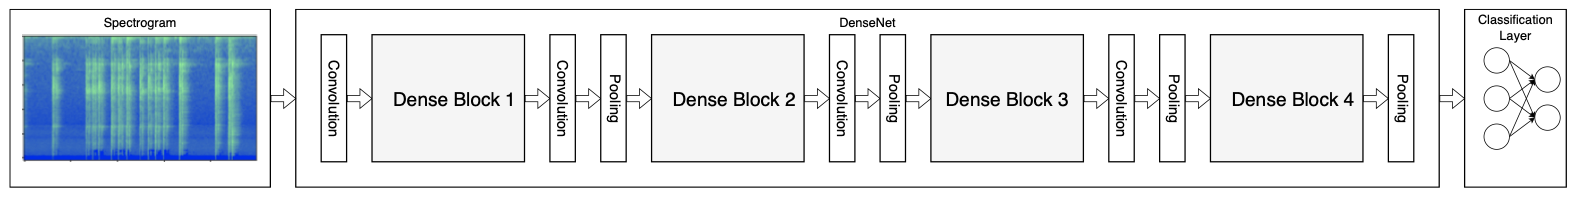
\includegraphics[scale=0.55]{pics/cnn_sound.png}
        \caption{Пример работы сети для классификации звука \cite{palanisamy2020rethinking}.}
        \label{cnn_sound}
    \end{figure}

    Алгоритм заключается в переводе звукового файла в спектрограмму и последующего применения сети \textbf{DenceNet} 
    \cite{huang2017densely} к полученному изображению. Ключевой особенностью этого подхода является то, что сама сеть никак 
    не модифицировалась. В итоге авторам удалось добиться лучшего качества на двух из трёх заявленных датасетах, используя 
    ансамбль свёрточных сетей (Рис. \ref{sound_res}a).

    Так же в работе изучалось изменение предобученных весов в сети по мере обучения (Рис. \ref{sound_res}b). Как оказалось, веса, находящиеся на начальных 
    слоях почти не претерпели изменений, в то время как веса, находящиеся на глубоких уровнях сети, сильно адаптировались под новые данные. 
    Эти выводы согласуются с нашими рассуждениями из раздела \ref{cnn_vis}, ведь на начальных слоях сеть запоминает простейшие абстракции, 
    такие как линии и изменения цвета, а на последних она хранит информацию о высокоуровневых объектах, например, о человеческом лице или 
    колесе автомобиля.

    \begin{figure}[ht]
        \centering
        \begin{subfigure}[b]{0.6\textwidth}
            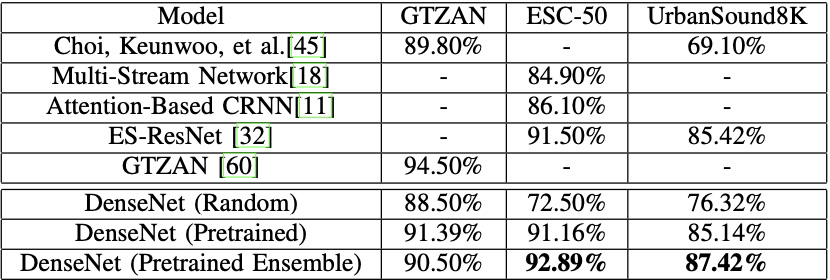
\includegraphics[width=\linewidth]{pics/sound_scores.png}
            \caption{сравнение ансамбля DenceNet с лучшими алгоритмами}
        \end{subfigure}
        \begin{subfigure}[b]{0.4\textwidth}
            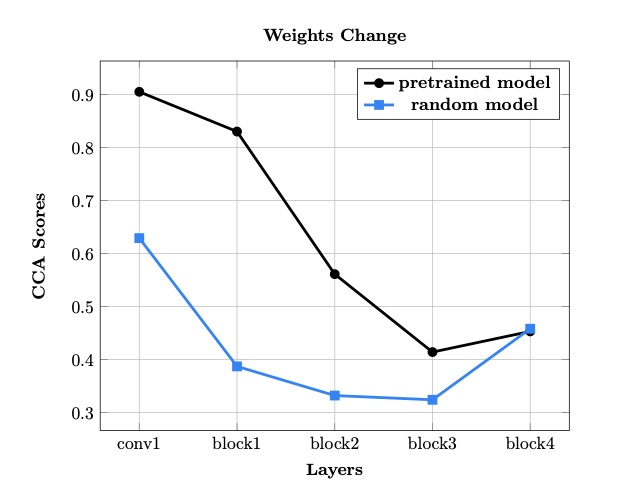
\includegraphics[width=\linewidth]{pics/sound_weights.png}
            \caption{корреляция весов со значениями до обучения}
        \end{subfigure}
        \caption{Изучение свойств DenceNet, обученной на спектрограммах \cite{palanisamy2020rethinking}.}
        \label{sound_res}
    \end{figure}  

    Таким образом, путём несложных преобразований, мы можем приспособить свёрточные сети для совершенно нового класса задач, главное 
    представить вход в нужном виде. В этом случае проблемы, перечисленные в предыдущем пункте, неактуальны, потому что спектрограммы~--- 
    это высокоточное признаковое описание звука, в котором невозможны смена перспективы или яркости.

    \subsection{Свёрточная сеть для изучения графов}

    Помимо модели применения поменялись также и сами архитектуры свёрточных сетей. Например, популярностью пользуется 
    сеть, созданная для предсказания дорожного трафика \cite{yu20193d}. В ней используется графовая свёртка
    \begin{equation} \label{1d_graph_conv}
        \hat{X} = U \Lambda_{\theta} U^T X,
    \end{equation}
    \noindent где $X \in \mathbb{R}^n$~--- входной графовый сигнал (вектор состояний вершин), 
    $U \in \mathbb{R}^{n \times n}$~--- матрица, содержащая базис из собственных векторов Лапласиана исходного графа, 
    $\hat{X} \in \mathbb{R}^n$~--- выход свёртки, $\Lambda_{\theta} \in \mathbb{R}^{n \times n}$~--- ядро свёртки, $n$~--- 
    количество вершин в графе.

    Подобный вид преобразования позволяет извлекать локальные признаки из графовой структуры. Также, так как $U$ зависит 
    только от вида самого графа, в процессе обучения мы ищем только значения диагональной матрицы $\Lambda_{\theta}$.

    \begin{figure}[ht]
        \centering
        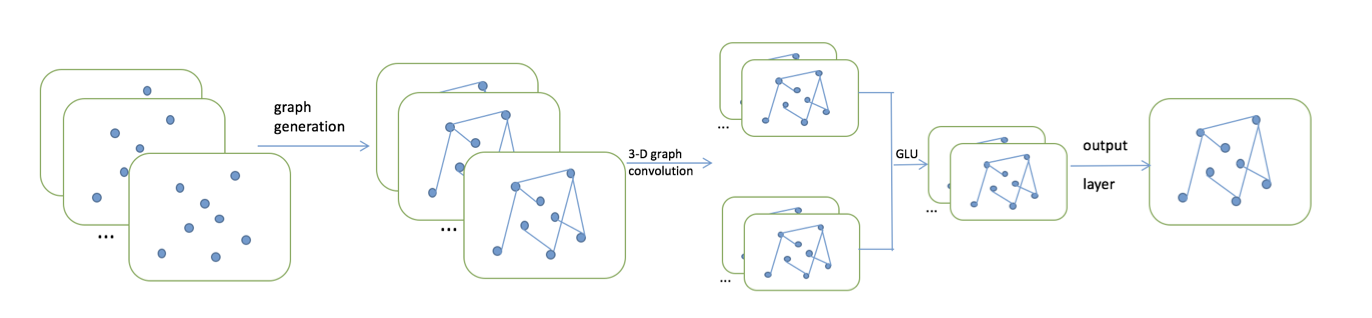
\includegraphics[scale=0.65]{pics/3D_TGCN.png}
        \caption{Архитектура графовой свёрточной сети \cite{yu20193d}.}
        \label{cnn_3d}
    \end{figure}

    Также стоит отметить, что в этой сети используется трёхмерная свёртка (координаты и время), свёртка (\ref{1d_graph_conv}) 
    применяется для каждого измерения. В отличие от предшественников, эта архитектура не пользуется априорной структурой 
    графа, а создаёт своё внутреннее представление на основе сравнения имеющихся маршрутов. Итоговый результат проходит 
    через пропускной линейный блок (\textit{Gated Linear Unit, GLU}).

    \section{Заключение}

    В этой работе мы изучили основные строительные блоки свёрточной нейронной сети, посмотрели на то, как эти блоки можно 
    настраивать и подумали о будущем этого сегмента глубокого обучения. Кроме того, мы затронули мотивацию тех или иных 
    составляющих сети и немного поговорили об интерпретируемости самой модели.

    Постепенно внимание сообщества переключается на более новые парадигмы, однако свёрточные сети всё ещё показывают лучшее 
    качество в области анализа изображений и плотно встроены в промышленную разработку. Помимо прочего, хоть и в задаче 
    анализа последовательностей их потеснили трансформеры, свёрточные сети широко используются при исследовании многомерных 
    объектов с локальными свойствами, например, графов.

    \newpage
    \bibliographystyle{unsrt}
    \bibliography{reference}
    
\end{document}
